%
%%
%%
%%

%% [intro]

Calibration of the flux density scale of the instrument NIKA2 in its final configuration
of January 24th 2017  is studied in this section  in using the 
 primary calibrators, Uranus and Neptune, and secondary calibrators, the two largest asteroids Ceres and Vesta, and the three
planetary nebulae NGC7027, CRL2688, and MWC349, observed during run 9.

\subsection{Reference flux densities of the calibrators}

The planets Uranus and Neptune are standard calibrators for many instruments,
{\it e.g.} PACS and SPIRES aboard Herschel and SCUBA2 at JCMT,
and their flux densities over a large spectrum from centimeter wavelengths to optical are provided by the model of Moreno et al (1998)
with an accuracy better than
5\% at millimeter wavelengths (Moreno, private communication). Flux densities provided by this model for
the reference angular sizes of $3.5''$
and $2.3''$ for Uranus and Neptune, respectively, have been  computed
for 24th february 2017 with their
distances provided by  the JPL ephemerides \footnote{https://ssd.jpl.nasa.gov/horizons.cgi}.
They were computed at the central frequencies of the bandpasses of
the three arrays (255 GHz, 152 GHz, 258 GHz) (EN REALITE, FAIT A (255+258)/2, A REFAIRE).

The asteroids Ceres and Vesta have been modeled by Muller et al (2014) accounting for 
size, shape, spin-properties, albedo, and thermal properties and adjusted to PACS, SPIRE and HIFI measurements
from Herschel to better than an accuracy of 5\%. 
Thomas Mueller has tabulated flux densities at different wavelengths, in particular at 1300$\mu$m, every five days
until 2020 \footnote{http://www.iram.es/IRAMES/mainWiki/Continuum/Calibrators}.
We have used the prediction at  1300$\mu$m made for  23rd february 2017
and extrapolated it  to the central frequencies of the arrays in using the Rayeigh-Jeans
spectrum expected for Ceres and Vesta. Their flux densities in
Table~\ref{tab:fluxPred} are for this data. Over the five days of  run 9 (february 23 - 28), the
flux densities  at 1300$\mu$m  have decreased by  3\% 
for Ceres and  by 6\%  for Vesta in Muller's tables but we have not corrected for this effect in our analysis below.  

The secondary calibrator MWC349A is a young Be star, part of a stellar binary system, surrounded by a disk. Its radio
continuum emission originates in an ionized bipolar outflow (Tafoya et al 2004).
MWC349 has been monitored with the  Plateau de Bure interferometer
and shown to be only slightly angularly resolved, making it a point source for the 30-metre telescope. We have adopted
its flux densities from this monitoring \footnote{http://www.iram.fr/IRAMFR/IS/IS2012/presentations/krips-fluxcalibration.pdf}.
The secondary calibrator CRL2688 is an Asympotic Giant Branch star. Its radio continuum emission is mostly from circumstellar dust and
is extended on a scale of $30''$ (Knapp et al 1994).
Its flux densities at $850\mu$m  and $450\mu$m  have been stable at the 5\% level as monitored between May 2011 and
May 2012 by SCUBA2 (Dempsey et al 2013).
we have extrapolated their flux densities at these two wavelengths and extrapolated to the central frequencies
of the arrays with a power law of index $\alpha=-2.47$.
The secondary calibrator NGC7027 is a young, dusty, carbon rich Planetary Nebula with an ionized core.
It is extended in the continuum and molecular lines (Bieging et al 1991) and  is not a point source for the telescope.
Its  most recent flux densities are reported at $1100\mu$m  and $2000\mu$m by Hoare et al (1992). It has been reported
to decrease by 0.145 percent/yr in the optically think regime at high frequencies ($> 6$GHz) at the VLA
(Zijlstra, van Hoof \& Perley 2008, and Hafez et al, 2008) that makes these flux densities uncertain by 3.6\%.  
Its SED from cm wavelength to optical is also presented in Hafez, Y.A. et al (2008).
The flux densities adopted at the central frequencies of the arrays for these three calibrators are in Table~\ref{tab:fluxPred}.


\begin{table}
\centering
\label{tab:fluxPred}
\caption[]{Reference flux densities of calibrators.}
\begin{tabular}{|l|c|c|c|}
\hline
\multicolumn{1}{|c}{}  & \multicolumn{3}{|c|}{flux densities (Jy)}  \\
\hline
         &    A1      &  A2   &   A3    \\
\hline
Uranus   &  37.36  & 16.40 &  37.38 \\
Neptune  &  15.31  &  6.87 &  15.31  \\
Vesta    &  0.99   &  0.35 &  0.99 \\
Ceres    &  0.89   &  0.31 &  0.89   \\
MWC349   &  2.2   &    1.6 &   2.2 \\
NGC7027  &  3.61   &  4.42 &  3.61 \\
CRL2688  &  3.03  &   0.83 &c 3.03  \\
\hline
\end{tabular}
%\label{tab:fluxPred}
\end{table}





\subsection{Aperture photometry}

The calibrators were observed frequently during run9. These observations were beammaps for Uranus and Neptune
along  with  sequences of 4 consecutive
otf maps ($8' \times 5'$) as for Ceres Vesta, NGC7027, CRL2688, and MWC349. All observations were processed with the pipeline in using
the kidpar {\it kidpar-best3files-FXDC0C1-GaussPhot}, line-of-sight opacities, and the standard
gain-elevation curve of the telescope to produce intensity maps for the three arrays.
Uranus and Neptune have a significantly larger flux densities than the other calibrators, and  are the best sources to caracterize the
instrument and calibrate the flux density  scale of the instrument,
in addition to the fact that their flux densities  are accurateky known.
The total flux densities of all ten observations of these planets in run 9 are in Table~\ref{tab:fluxAp} as
measured directly with aperture photometry over a large radius of 150'' to include the most significant part of the
error beam and reach saturation.  These flux density measurements are are of high quality over a broad range of observing conditions
($33^{\circ}<$ elevations $<58^{\circ}$, and   $0.16 < \tau_{1mm} < 0.50$, see details in  Table~\ref{tab:fluxAp}). An illustration of
such a high quality aperture photometry is in Fig.~\ref{fig:PhAp}.

An important step in the flux density measurement from each map is the estimation of the solid angle of the true beam, {\it i.e.} main beam
and side lobes, so that intensity in each pixel chosen to be $1'' \times 1''$ in size in our process can be calculated prior to summation for
aperture photometry. We have computed the true beam as $ \Omega_{true} (r_{max}) = \int_0^{2\pi} \int_0^{r_{max}} B(r) 2 \pi r dr$ where
$B(r)$ is the radial profile of the azimuthally averaged brigthness over annuli $dr$ wide, and normalised so that B(0)=1.
(SEE WEIGHTED MEAN). We have used  $r_{max}=250''$ but  $ \Omega_{true}$ saturates at $r_{max}=150''$ as illustrated
in Fig.~\ref{fig:PhAp}. This expression is similar
to the one used in Adam (2016)  (\S 8.1.1.2 in PhD thesis) but is for a  brightness distribution assumed azimuthally symmetric. 
The excess
of the true beam relative to the Gaussian beam is $\Omega_{true} / 2 \pi (\sigma_{Gauss})^2$ where  $\sigma_{Gauss}$ is from
$FWHM$ estimated for each observation as described in section ???.  (ADD TABLE WITH $FWHM$, $\Omega_{Gauss}$ and $\Omega_{true}$).
%In Table~\ref{tab:Omegatrue}, these excesses are reported
%as well as $FWHM$, $\Omega_{Gauss}$ and $\Omega_{true}$  for the ten observations
%of Uranus and Neptune.
For the ten observations of Uranus and Neptune, means and rms of the excesses
are $1.72 \pm 0.12 $, $ 1.33 \pm 0.04$, and $1.68\pm 0.13 $ for arrays A1, A2 and A3, and medians are 1.835, 1.370, and 1.784.
These excesses were 1.34 and 1.28 at 1mm and 2mm, respectively, for NIKA (Adam 2016). These excesses reflect  the
residual side lobes left after correction of the data with the standard gain curve of the telescope (...REFERENCE...) used in the processsing 
with the pipeline as mentioned above. Had we turned off this gain correction,  $\Omega_{true}$ would have been a function of the
elevation.



\begin{table}
\centering
\label{tab:fluxAp}
\caption[]{Measured flux densities of primary calibrators.}
\begin{tabular}{|l|c|c|c|c|c|c|c|}
\hline
\multicolumn{1}{|c}{} & \multicolumn{1}{|c}{ observation}  & \multicolumn{1}{|c}{elev. ($^{\circ}$) } &  \multicolumn{1}{|c}{$\tau_{1mm} $}  &  \multicolumn{1}{|c}{$\tau_{2mm} $ } & \multicolumn{3}{|c|}{flux densities (Jy)}  \\
\hline
&                   &             &                &                 &    A1              &  A2   &   A3    \\
\hline
 Uranus   & 20170223s46  &  37.9 & 0.48 & 0.31 & $     35.18 \pm        1.61$  & $     16.57 \pm        0.41$ & $     37.26 \pm       1.19$  \\
 Neptune  & 20170224s177 &  39.2 & 0.50 & 0.34 & $     15.85 \pm        1.03$  & $      7.43 \pm        0.20$ & $     16.45 \pm       0.82$  \\
 Uranus   & 20170225s222 &  35.6 & 0.28 & 0.18 & $     38.54 \pm        0.77$  & $     16.71 \pm        0.24$ & $     39.05 \pm       0.66$  \\
 Uranus   & 20170225s266 &  58.2 & 0.28 & 0.19 & $     39.25 \pm        0.62$  & $     16.69 \pm        0.17$ & $     39.58 \pm       0.50$  \\
 Uranus   & 20170227s308 &  56.1 & 0.17 & 0.14 & $     37.02 \pm        0.63$  & $     16.35 \pm        0.25$ & $     38.62 \pm       0.58$  \\
 Uranus   & 20170227s304 &  57.7 & 0.16 & 0.13 & $     36.39 \pm        0.45$  & $     16.17 \pm        0.16$ & $     36.87 \pm       0.39$  \\
 Uranus   & 20170227s315 &  51.3 & 0.19 & 0.15 & $     36.85 \pm        0.52$  & $     16.65 \pm        0.15$ & $     38.49 \pm       0.46$  \\
 Uranus   & 20170227s321 &  46.6 & 0.18 & 0.14 & $     35.69 \pm        0.58$  & $     16.33 \pm        0.16$ & $     37.78 \pm       0.52$  \\
 Uranus   & 20170227s352 &  36.9 & 0.23 & 0.17 & $     33.35 \pm        0.66$  & $     17.11 \pm        0.17$ & $     32.30 \pm       0.55$  \\
 Uranus   & 20170227s356 &  33.9 & 0.22 & 0.17 & $     36.01 \pm        0.72$  & $     16.78 \pm        0.18$ & $     36.75 \pm       0.64$  \\
\hline
\end{tabular}
%\label{tab:fluxAp}
\end{table}



\begin{figure}
\begin{center}
  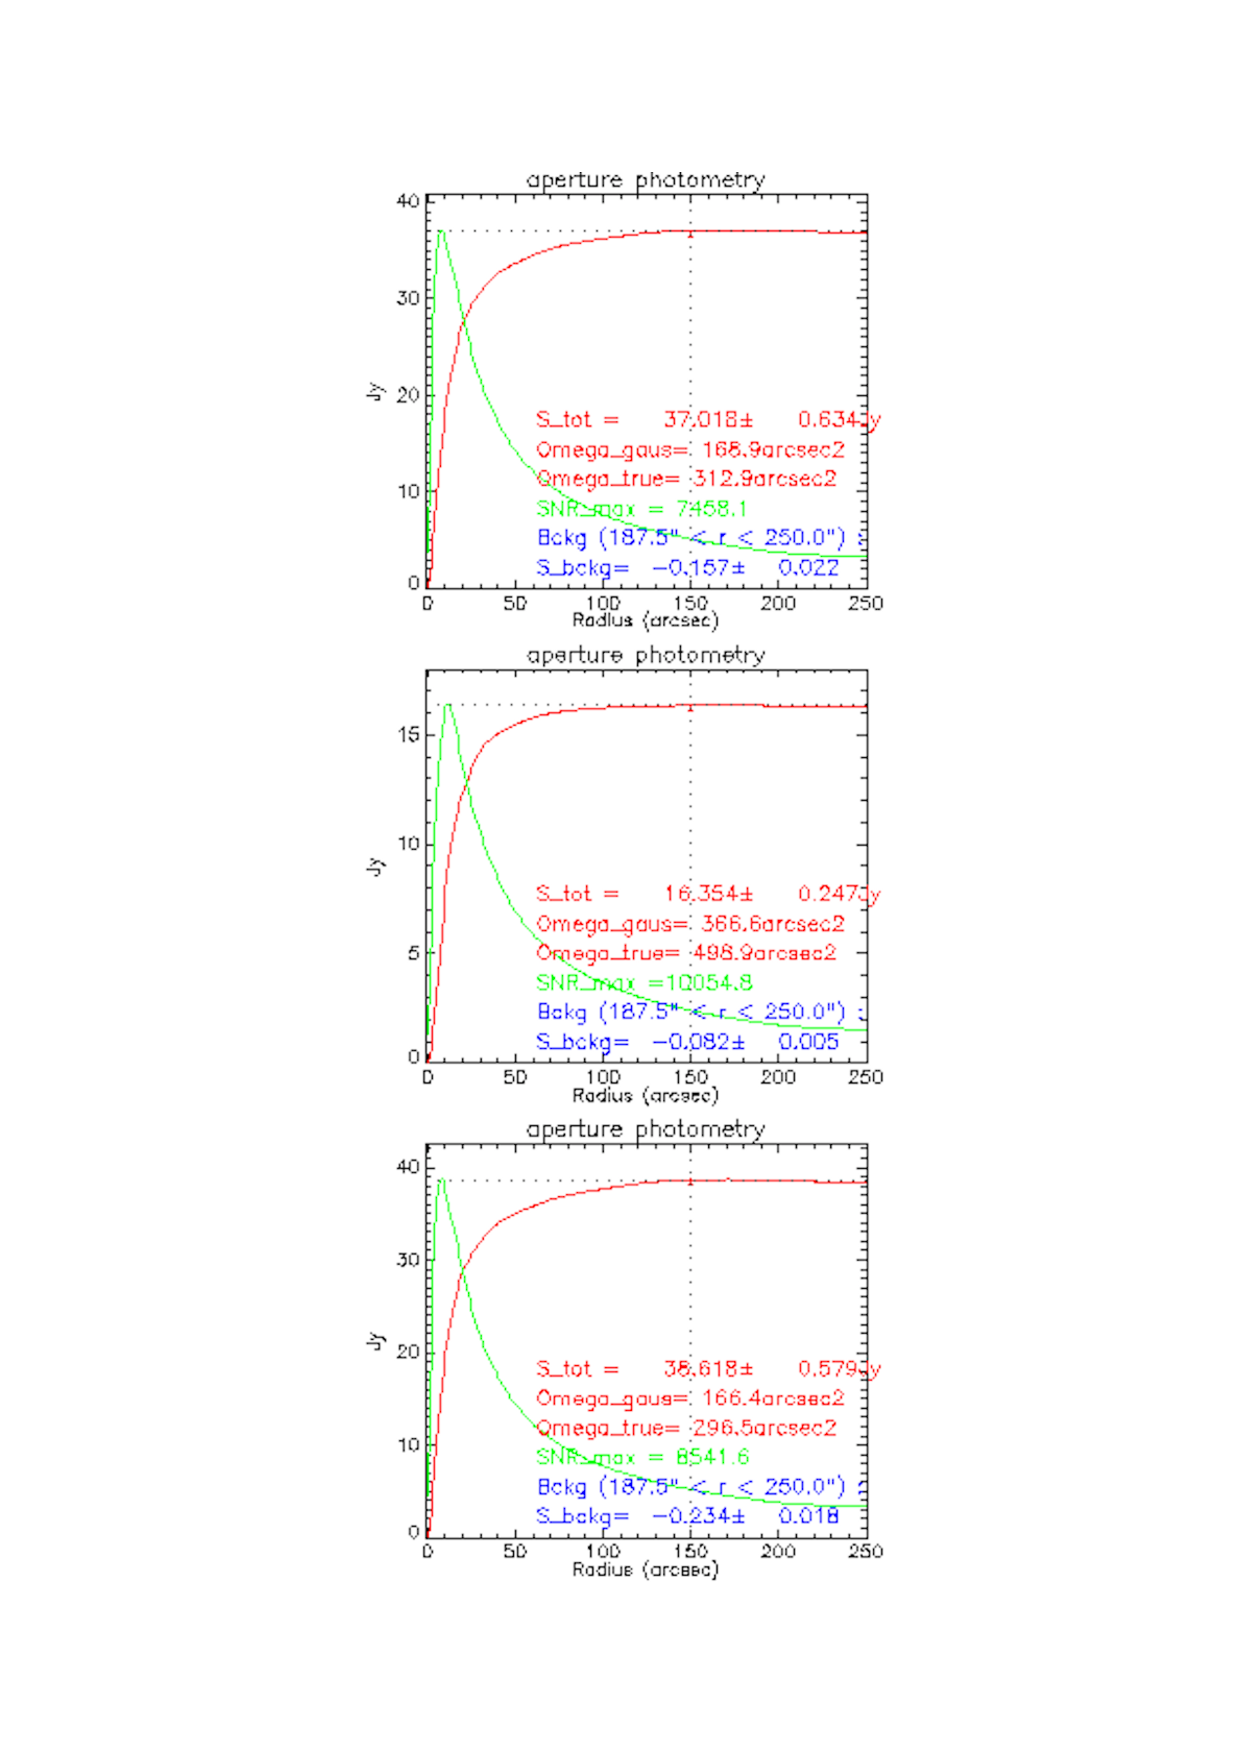
\includegraphics[clip, angle=0, scale=0.4]{Figures/Uranus_s308.pdf}
  \caption{Aperture photometry of Uranus observation 20170227s308  on array 1, 2 and 3 from top to bottom.
    The photometric curve in red saturates at about the radial distance of $150''$ from the
    source brightness center with a precision of a small fraction of Jy. (Green curve is the SNR in individual annulus but can be ignored for this
  presentation; WILL BE DELETED FOR FINAL DRAFT)}
\label{fig:PhAp}
\end{center}
\end{figure}

We compare now the measured and reference flux densities of the planets given in Tables~\ref{tab:fluxAp} and ~\label{tab:FluxPred}
in plotting their  ratios in Fig.~\ref{fig:U_N_ratio} that are found  unity within 4.6 \% for array A1,  2.5 \% for array A2, and
5.5 \% for array A3. Hence,
the absolute calibration over these ten observations of the primary calibrators is consistent with the uncertainty of $< 5\%$
claimed for the model of Moreno et al.




\begin{figure}
\begin{center}
  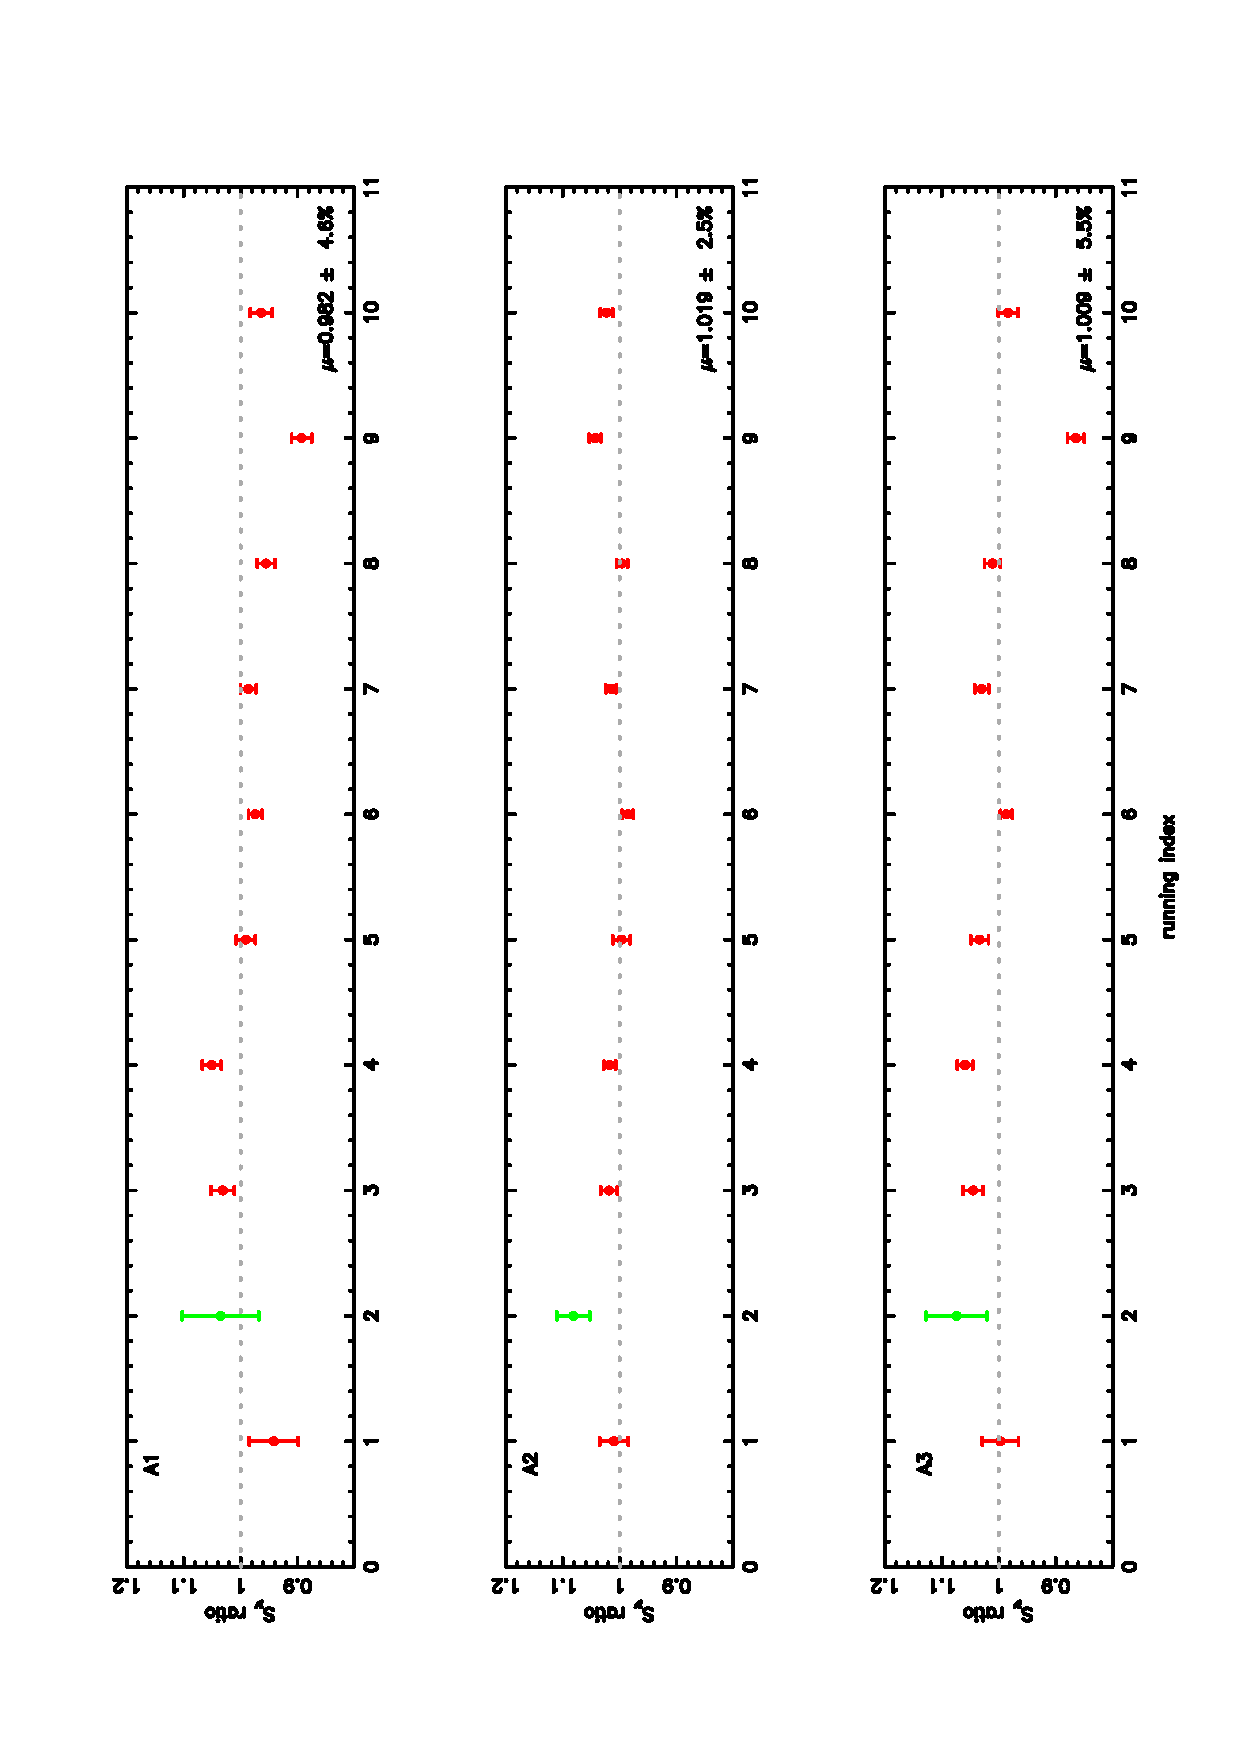
\includegraphics[clip, angle=-90, scale=0.6]{Figures/ratio_Ura_Nept.pdf}
  \caption{Comparison between the measured and reference flux densities for all observations of Uranus and Neptune during run 9
    for the three arrays. Red is for Uranus and Green is for Neptune.}
\label{fig:U_N_ratio}
\end{center}
\end{figure}



As already mentioned, estimation of these measured flux densities comprises  the true beam $\Omega_{true}$ from each map
because the planets  are uncommonly  strong sources for which this calculation is accurate enough.
For sources less than 1 Jy, this cannot be done and $\Omega_{true}$ must be estimated from $\Omega_{Gauss}$
in using a fixed excess factor for each array. We have derived these factors in re-estimating 
the flux densities of the planets for all observations of run 9 in  using  $\Omega_{Gauss}= {2 \pi \over (2 \sqrt{2 ln 2})^2} \times (\rm FWHM)^2$
with the FWHM of the main beam estimated from each map.  These 
factors are  1.927 for arrays A1 and A2, and 1.440 for array A2, so that the mean flux density ratio is unity for each array  as
shown in Fig.~\ref{fig:U_N_ratio_fixed}. These factors are slightly larger than the means and medians of $\Omega_{true}/\Omega_{Gauss}$
determined above that, if used, slightly over estimate flux densities. With this approach,
the absolute calibration over the ten observations of the primary calibrators
during run 9 is at a level of  8.0\% for array A1,  2.1\% for A2 and  9.7\% for A3. Hence, stability of absolute calibration
is somewhat degraded at 1mm, and similar at 2mm
relative to absolute calibration when the true beams $\Omega_{true}$ from individual maps are used. We stress that all ten observations
of the planets were used for this comparison ; in other words, no selection was applied, no observation was discarded as outlier.

Finally, we have plotted the flux density ratios versus elevation, line-of-sight opacities at 1mm and 2mm, and airmass
in Fig.~\ref{fig:U_N_versus}, and found no apparent correlation.




\begin{figure}
\begin{center}
  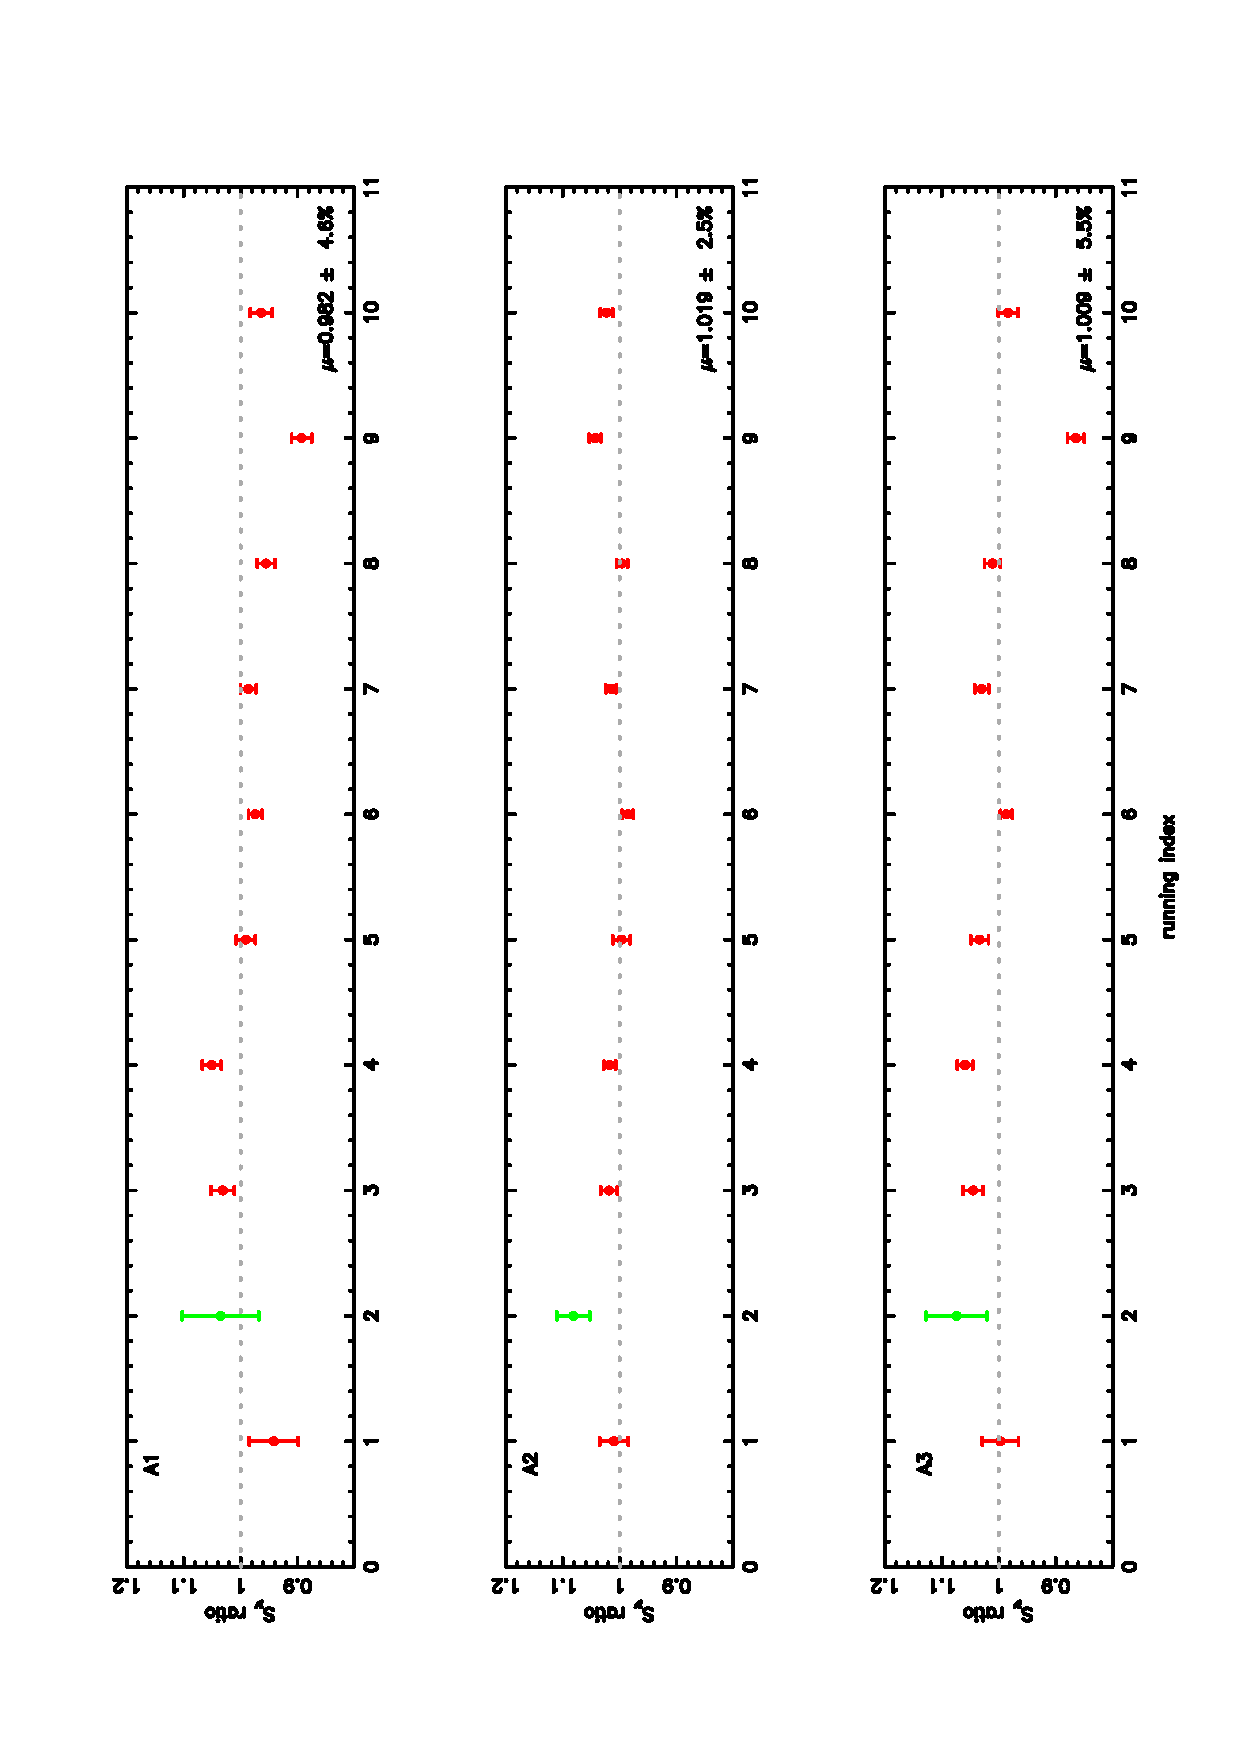
\includegraphics[clip, angle=-90, scale=0.6]{Figures/ratio_Ura_Nept.pdf}
  \caption{Comparison between the measured and reference flux densities for all observations of Uranus and Neptune during run 9
    for the three arrays.}
\label{fig:U_N_ratio}
\end{center}
\end{figure}


\begin{figure}
\begin{center}
  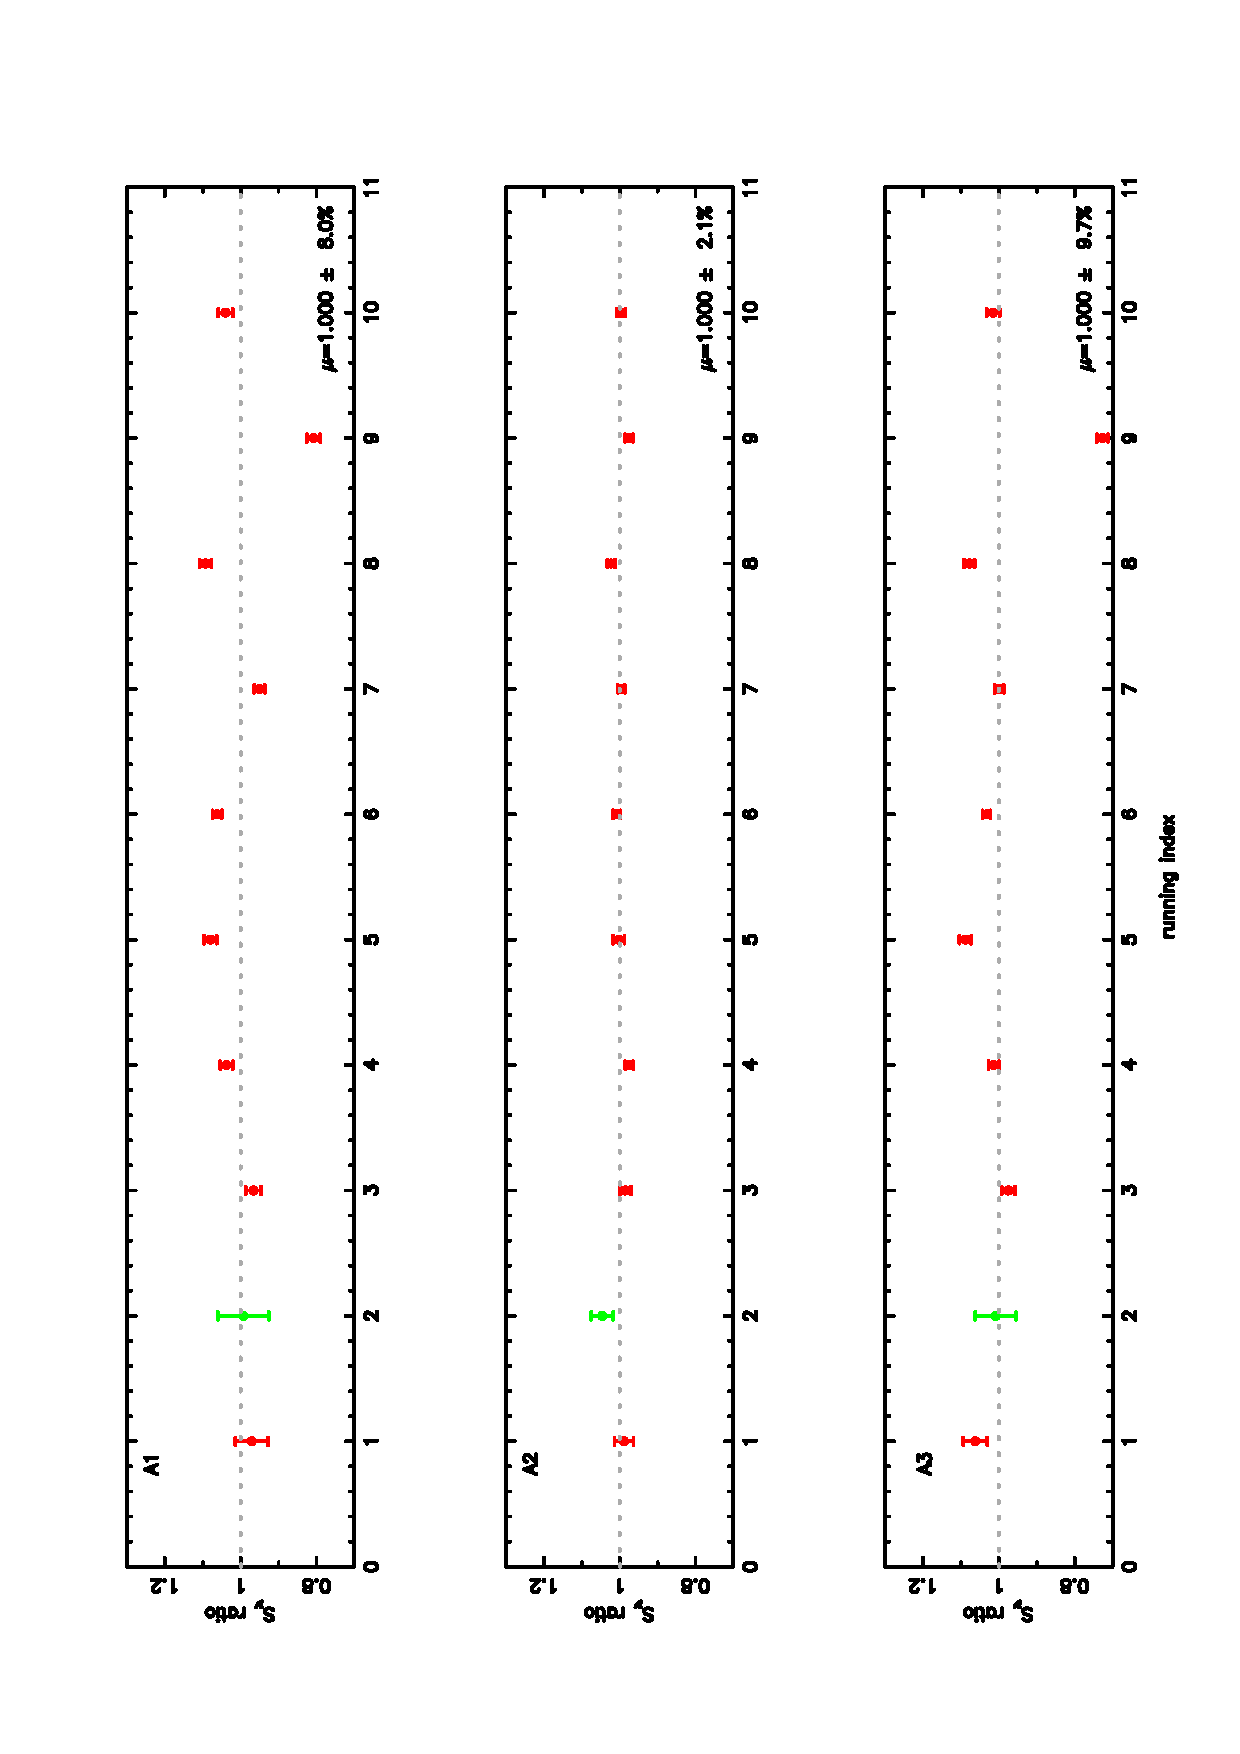
\includegraphics[clip, angle=-90, scale=0.6]{Figures/ratio_Ura_Nept_O_fixed.pdf}
  \caption{Same as Fig.~\ref{fig:U_N_ratio} but the solid angle of the true beam  $\Omega_{true}$
    is the  Gaussian beam $\Omega_{Gauss}$ scaled by the factors 1.927 for arrays A1 and A3, and 1.440 for array A2.
    The absolute calibration uncertainty is somewhat degraded at 1mm but similar at 2 mm when compared to previous Figure.
    Note that the vertical scale is different.
   }
\label{fig:U_N_ratio_fixed}
\end{center}
\end{figure}


\begin{figure}
\begin{center}
  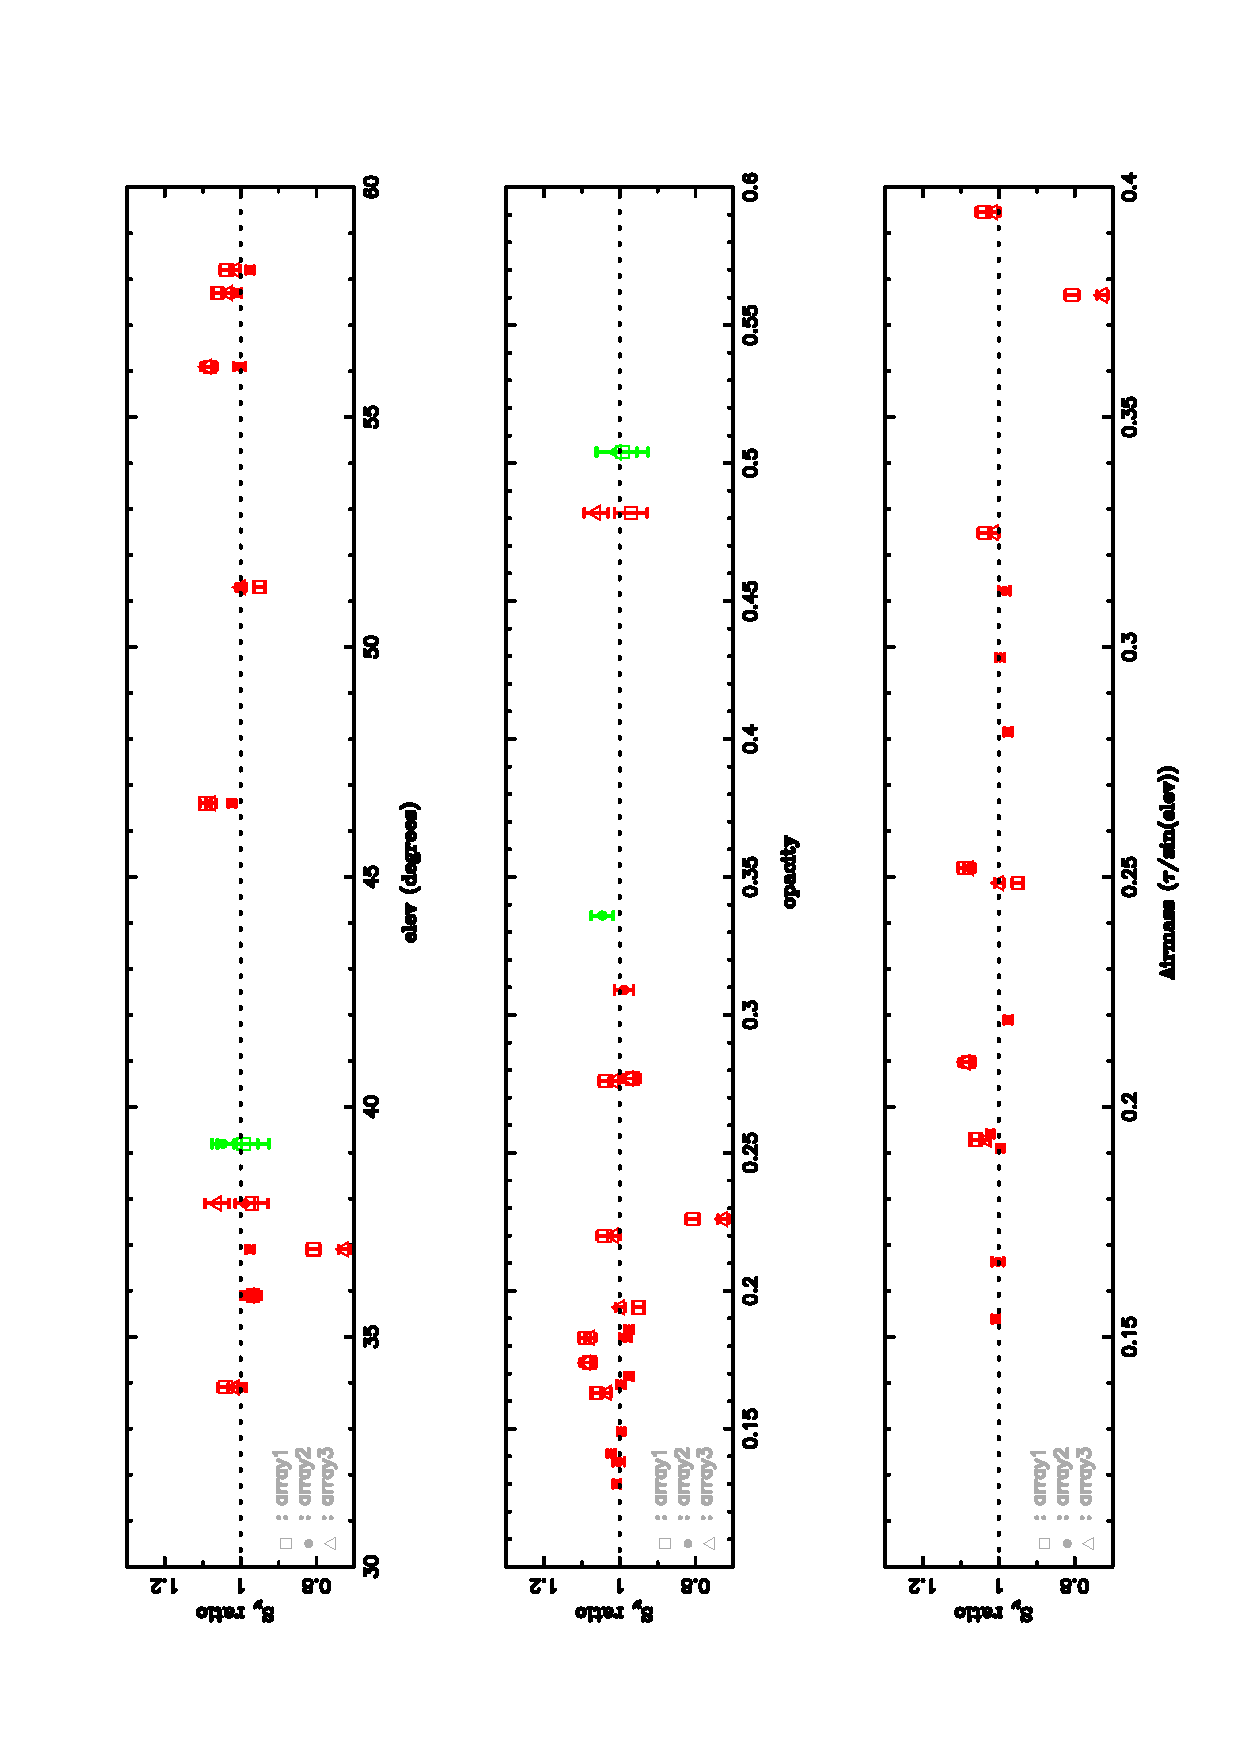
\includegraphics[clip, angle=-90, scale=0.6]{Figures/U_N_versus.pdf}
  \caption{Flux ratios versus elevations, opacities at 1mm and 2 mm, and airmass. No correlation is
    apparent.   }
\label{fig:U_N_versus}
\end{center}
\end{figure}






We have extended this  analysis to all the secondary calibrators (Ceres, Vesta, NGC7027, MWC349, CRL2688)
observed during run 9. As for the planets, the observations were processed with the pipeline including line-of-sight opacity.
Aperture photometry was carried out and the solid angle $\Omega_{true}$  estimated from each map,
except for Ceres and Vesta which are too faint. Four observations of secondary calibrators were discarded because
aperture photometry failed to converge. The fifty three observations remaining provided flux densities on the three
arrays that were compared to their reference flux densities given in Table~\ref{tab:fluxPred}. Their  ratios
 were plotted in Fig.~\ref{fig:all} in time order.
The eleven flux density  measurements of CRL2688 were all clearly too high  and were multiplied
by the factors 0.9 at 1mm and 0.75 at 2mm to yield the ratios shown in Fig.~\ref{fig:all}. Also, the flux density of Ceres at 1mm
in Table~\ref{tab:fluxPred} is too low  but we did not correct for it because the flux densities of the four observations
of Ceres have large uncertainties. This is apparent in the plot. The first obsertions of the strong source
Uranus (index 1 in plot) and Neptune (index 11 in plot) in mediocre weather during the first half of the run
do not show any degradation in the plot while secondary calibrators do. Overall,  the observations of
all calibrators, primary and secondary, with minimal selection (four discarded out of fifty seven) and 
a simple adjustement for calibrator CR2688, yield an absolute calibration stable  at the level
of 14\% for array A1, 8.1\% for array A2, and 16.7\% for array A3, during run 9
in  Fig.~\ref{fig:all}. In addition, no correlation is apparent with opacities, elevation, or airmass
as shown in  Fig.~\ref{fig:versus_all}.



\begin{figure}
\begin{center}
  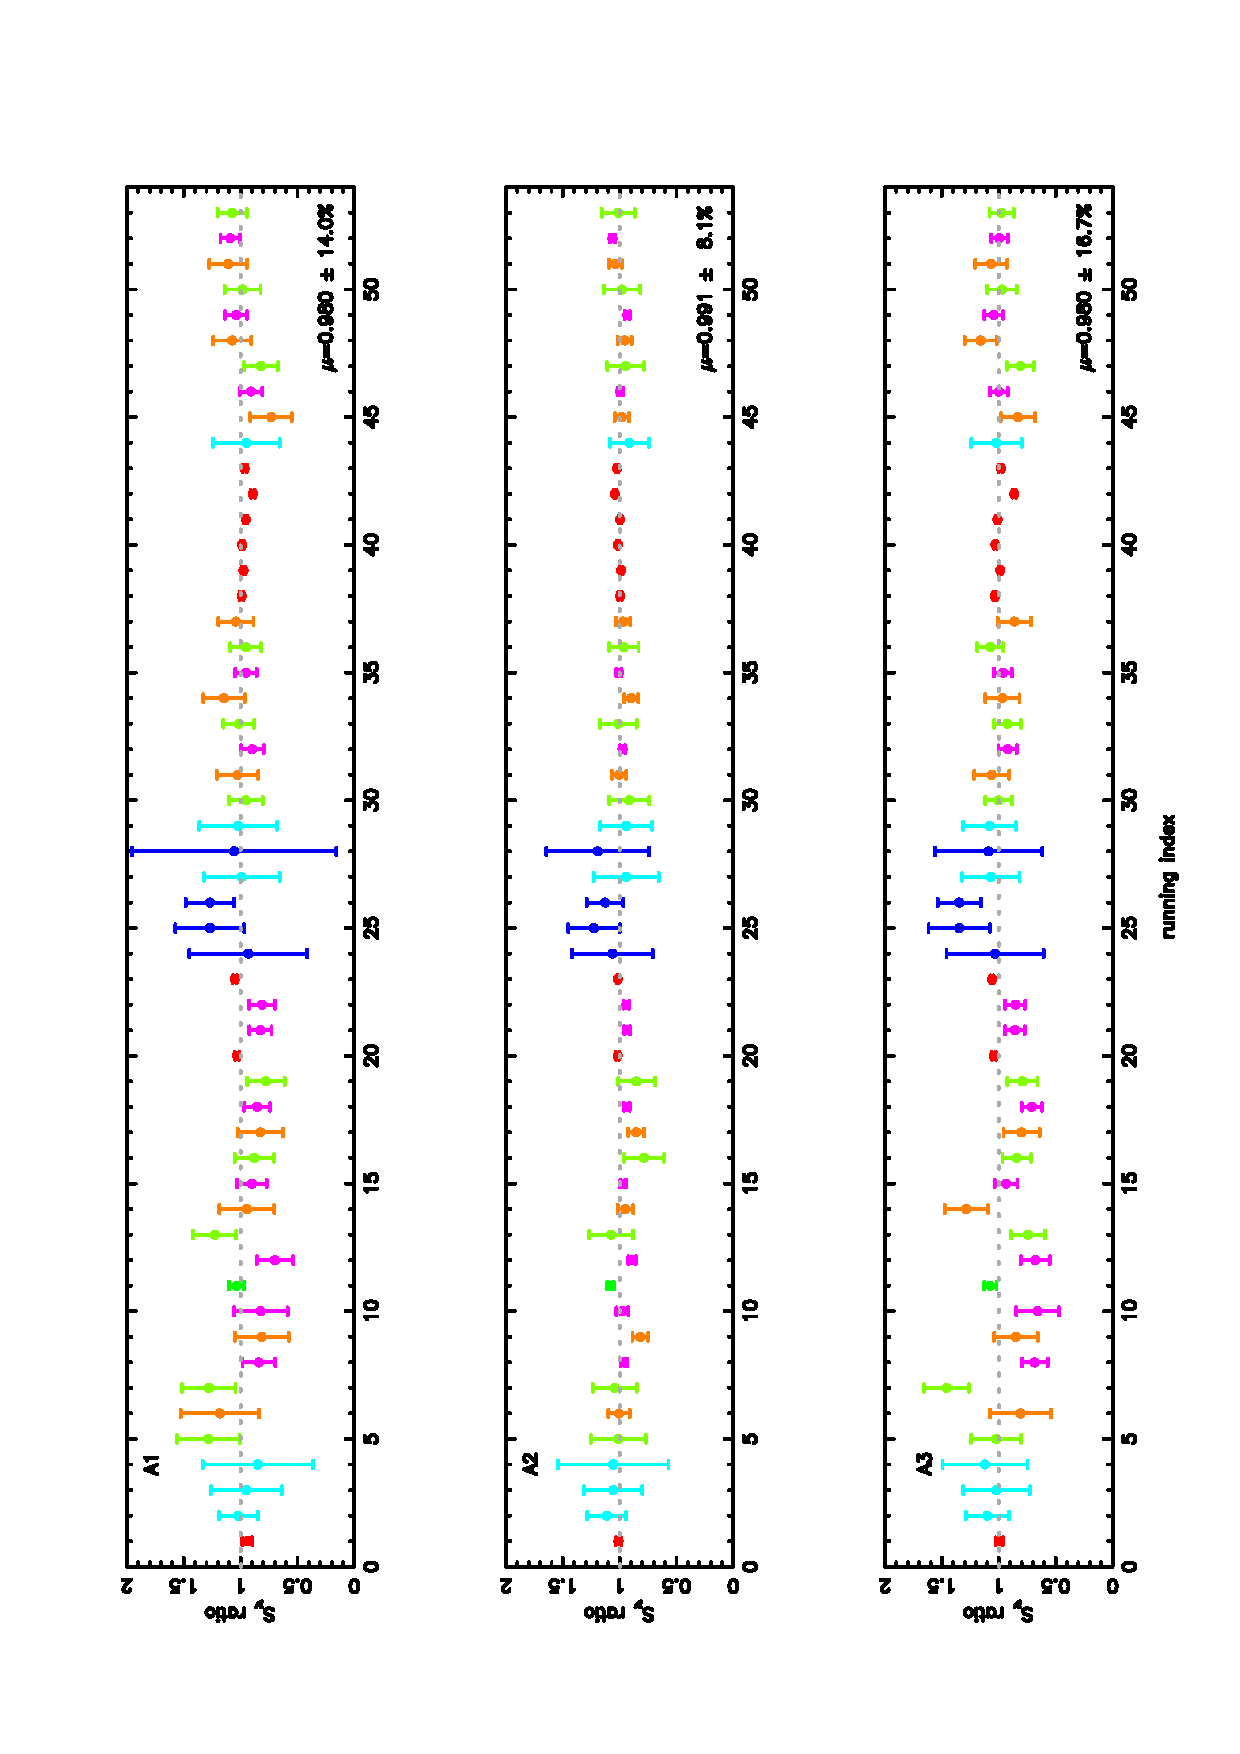
\includegraphics[clip, angle=-90, scale=0.6]{Figures/ratio_all.pdf}
  \caption{Comparison between the measured and reference flux densities for all primary and secondary calibrators  during run 9
    for the three arrays. Color codde is : Uranus (red), Neptune (darl green), Ceres (dark blue), Vesta (light blue), NGC7027 (magenta), MWC349 (brown),
    CRL2688 (light green). Running indices  are time-ordered. Weather conditions were mediocre during the first half of the run, improving
  drasticly in the second half.}
\label{fig:all}
\end{center}
\end{figure}

\begin{figure}
%\begin{center}
  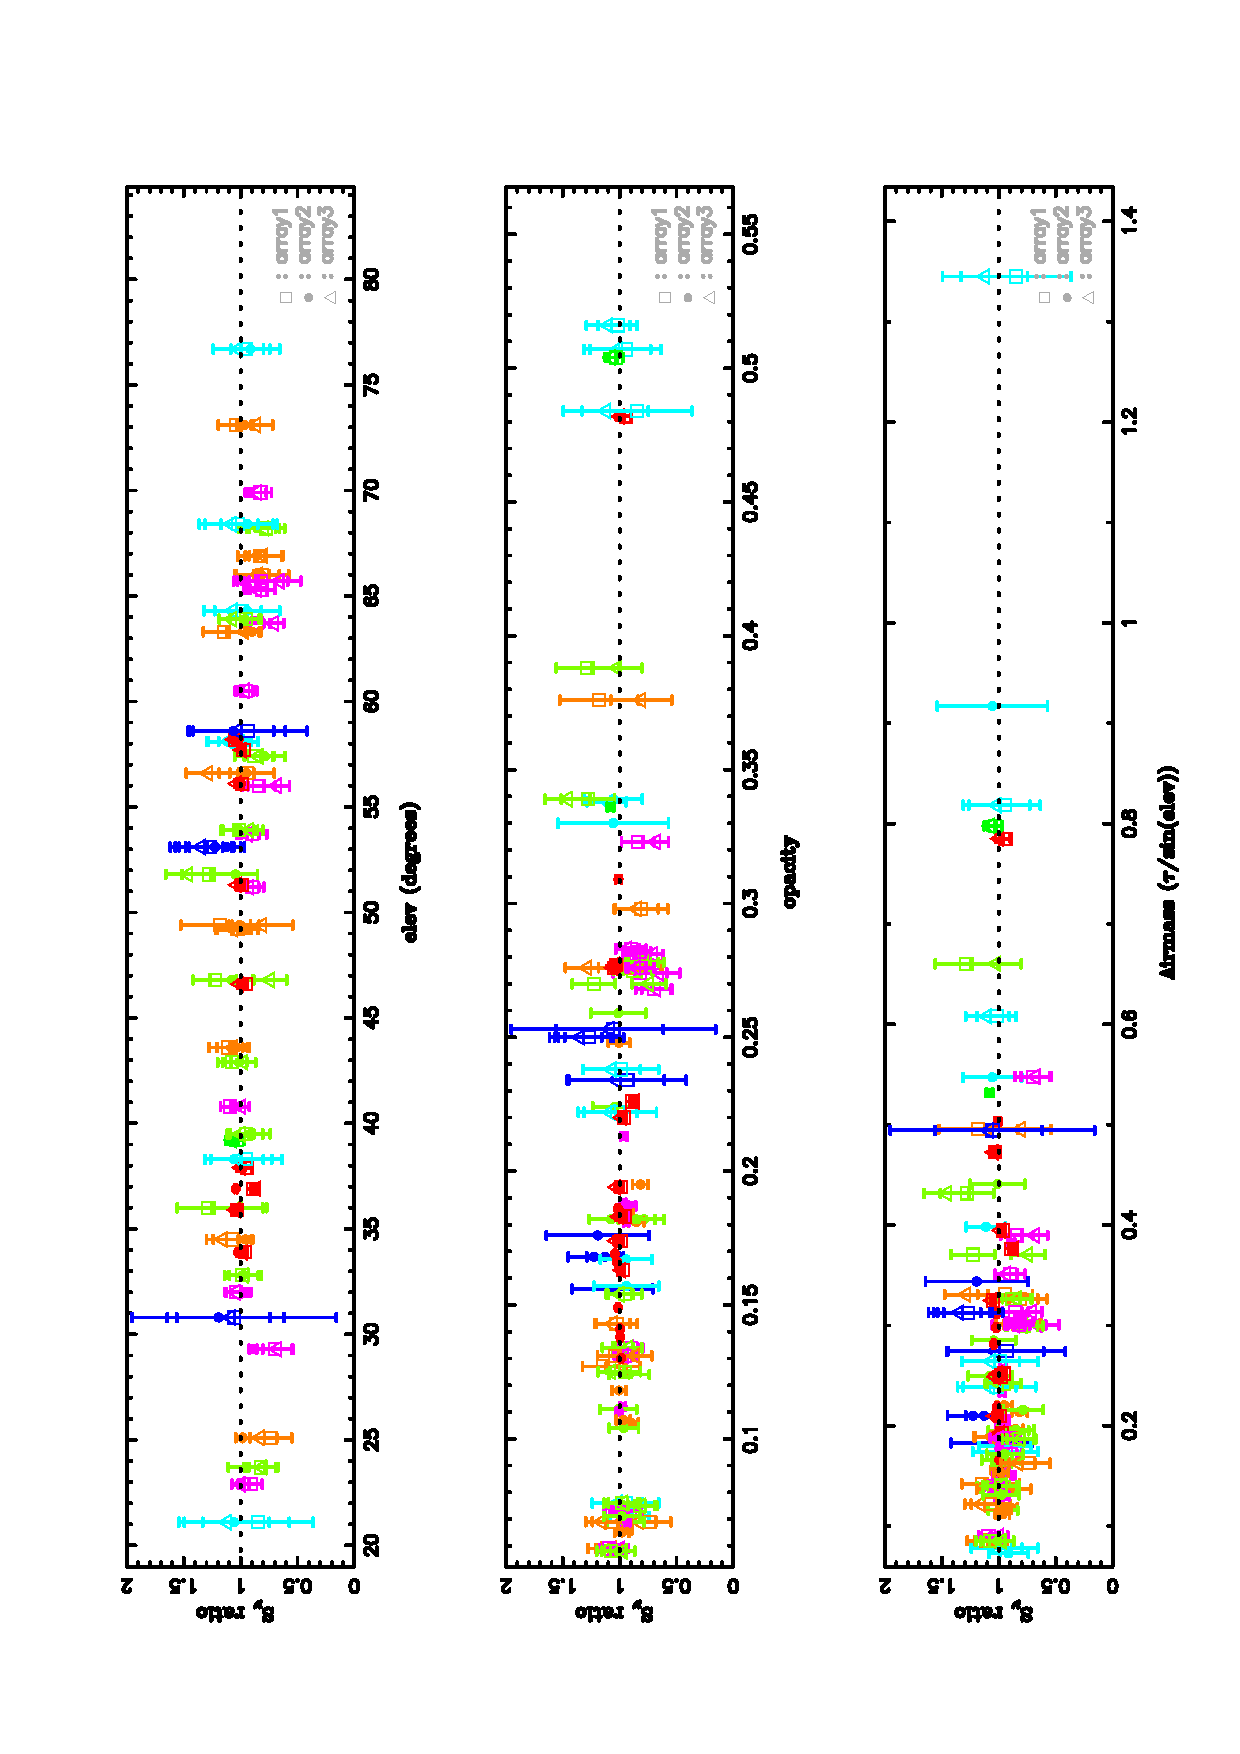
\includegraphics[clip, angle=-90, scale=0.6]{Figures/ratio_versus_all.pdf}
  \caption{Flux density ratios versus elevations, opacities at 1mm and 2 mm, and airmass. No correlation is
    apparent. Color code is same as in Fig.\ref{fig:U_N_versus}. }
\label{fig:versus_all}
%\end{center}
\end{figure}

\begin{figure}
%\begin{center}                                                                                                                                               
  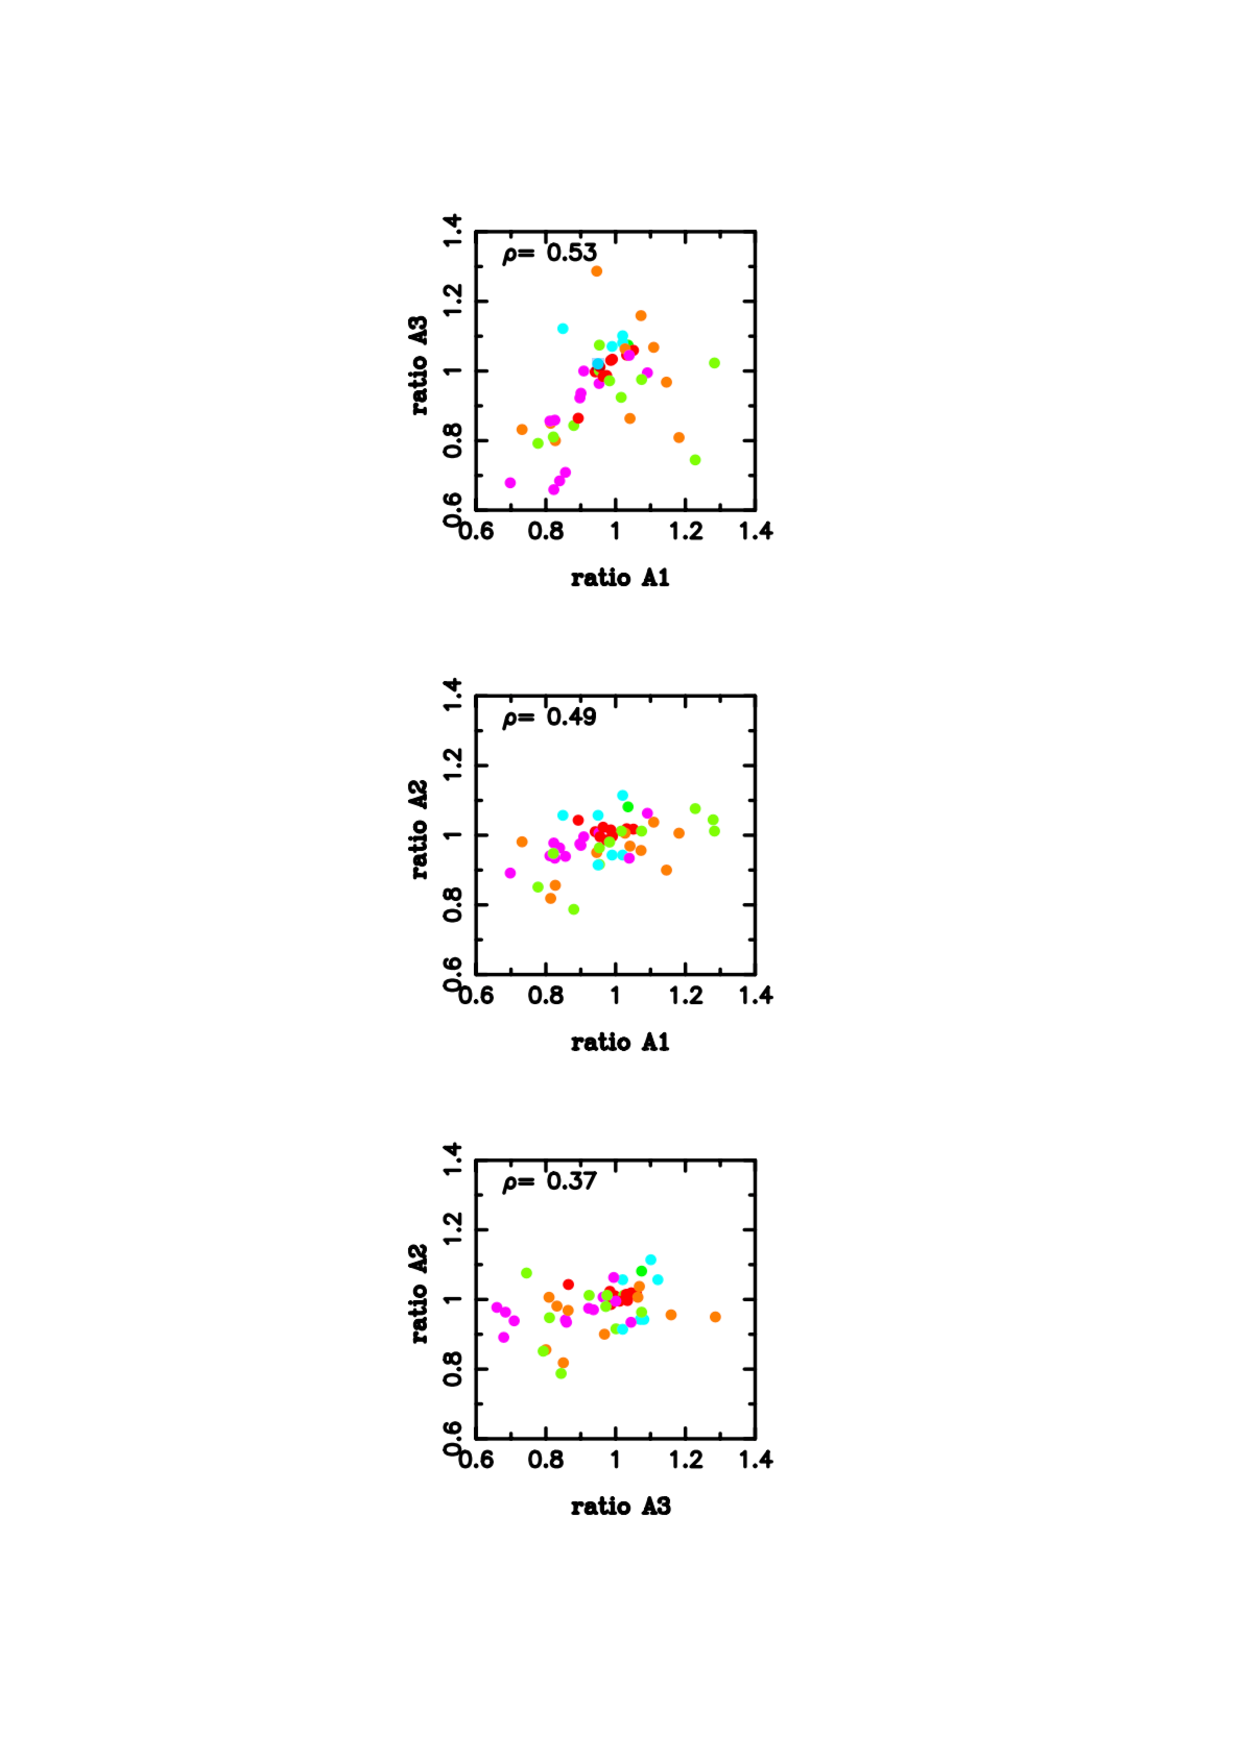
\includegraphics[clip, angle=0, scale=0.6]{Figures/correlation.pdf}
  \caption{Correlation between  flux density ratios of the three arrays for all calibrators.}
\label{fig:versus_all}
%\end{center}                                                                                                                                                 
\end{figure}











Correlation between arrays







